\documentclass[11pt,a4paper]{article}

% ---------------------------------------------------------------------------
%  Tahoe meshfree Kirchhoff--Love shell (RKShellT) -- Technical Report
%  Build:  make        (or)   latexmk -pdf technical_report.tex
% ---------------------------------------------------------------------------

\usepackage[margin=1in]{geometry}
\usepackage{lmodern}
\usepackage[T1]{fontenc}
\usepackage{amsmath,amssymb,bm}
\usepackage{mathtools}
\usepackage{graphicx}
\usepackage{booktabs}
\usepackage{array}
\usepackage{xcolor}
\usepackage{listings}
\usepackage{seqsplit}
\usepackage{enumitem}
\usepackage[hidelinks]{hyperref}
\usepackage{caption}

% --- notation macros --------------------------------------------------------
\newcommand{\dd}{\,\mathrm{d}}
\DeclareMathOperator{\tr}{tr}
\newcommand{\bsig}{\bm{\sigma}}
\newcommand{\bx}{\bm{x}}
\newcommand{\bX}{\bm{X}}
\newcommand{\bu}{\bm{u}}
\newcommand{\bd}{\bm{d}}
\newcommand{\bn}{\bm{n}}
\newcommand{\bB}{\bm{B}}
\newcommand{\bD}{\bm{D}}
\newcommand{\bC}{\mathbb{C}}
\newcommand{\bxi}{\bm{\xi}}
\DeclareRobustCommand{\code}[1]{\texttt{\seqsplit{#1}}}

% --- code listing style -----------------------------------------------------
\definecolor{codekw}{rgb}{0.13,0.29,0.53}
\definecolor{codecm}{rgb}{0.40,0.45,0.45}
\definecolor{codebg}{rgb}{0.97,0.97,0.97}
\lstset{
  basicstyle=\ttfamily\small,
  keywordstyle=\color{codekw}\bfseries,
  commentstyle=\color{codecm}\itshape,
  backgroundcolor=\color{codebg},
  frame=single, rulecolor=\color{gray!40},
  breaklines=true, showstringspaces=false,
  language=XML, captionpos=b, columns=fullflexible,
}

\title{\textbf{A Meshfree Reproducing-Kernel Kirchhoff--Love Shell in Tahoe}\\[4pt]
  \large Formulation, Implementation, Boundary Conditions, and Verification\\
  \large against Wang \& Bazilevs (2025)}
\author{Saman Seifi}
\date{\today \\[6pt] \small Technical Report --- Tahoe \code{develop}, issues \#59--\#73}

\begin{document}
\maketitle

\begin{abstract}
This report documents \code{RKShellT}, a rotation-free meshfree Kirchhoff--Love (KL) shell element
added to the Tahoe finite-element framework. The element follows the reproducing-kernel particle
method (RKPM) formulation of Wang and Bazilevs~\cite{WangBazilevs2025}: point-cloud geometry
through local principal-component charts, quadratic RK approximation with a cubic B-spline kernel,
nodal integration with Taylor-series (natural) stabilization, three-point through-thickness
integration of a plane-stress $J_2$ plasticity model, co-rotational stress update and a thickness
update. Two essential-boundary-condition treatments are provided for the non-interpolatory field:
direct nodal collocation and a new variational penalty controller that reports the physical
reaction. The element is verified against the Belytschko shell obstacle course and validated
against the elasto-plastic examples of the reference paper. With the current code, the
Scordelis--Lo roof reproduces the paper's four-mesh convergence to three digits, the necking
cylinder follows the paper's stabilized load curve within 1--4\% through the peak and into
softening, and the elasto-plastic pinched cylinder lies inside the published band once the
published curves are recognized to plot the symmetry-model load, one quarter of the physical
point load. Remaining limitations and the test infrastructure are summarized at the end.
\end{abstract}

\tableofcontents
\clearpage

% ===========================================================================
\section{Introduction and scope}\label{sec:intro}

Thin structures under large deformation, folding and self-contact are a natural target for
meshfree methods: the approximation is smooth, refinement does not need a conforming mesh, and
higher-order continuity is available without the $C^1$ element constructions that finite-element
Kirchhoff--Love shells require. Wang and Bazilevs~\cite{WangBazilevs2025} proposed a
general-purpose meshfree KL shell built on RKPM, and demonstrated it on the elastic obstacle
course, geometric accuracy on a point cloud, necking of a cylindrical shell, and the elasto-plastic
pinched cylinder.

This report describes the implementation of that formulation in Tahoe (GitHub epic \#59 and
sub-issues \#60--\#73), the boundary-condition machinery that a non-interpolatory field needs, and
the evidence that the implementation reproduces the paper. It supersedes the earlier working
notes in \code{docs/meshfree\_kl\_shell/} where they disagree; those notes are kept for history.

Units follow the reference paper: the elastic benchmarks use the consistent unitless data of the
obstacle course, and the elasto-plastic cases use millimetres, megapascals and newtons (density in
tonne/mm$^3$).

% ===========================================================================
\section{Formulation}\label{sec:formulation}

\subsection{Kinematics}
The shell is described by its mid-surface $\bar\bx(\xi^1,\xi^2)$ and unit normal $\bn$; a material
point at through-thickness coordinate $\xi^3\in[-1,1]$ sits at
\begin{equation}
  \bx(\xi^1,\xi^2,\xi^3) = \bar\bx(\xi^1,\xi^2) + \xi^3\,\frac{h}{2}\,\bn(\xi^1,\xi^2),
  \qquad \bn = \frac{\bar\bx_{,1}\times\bar\bx_{,2}}{\lVert \bar\bx_{,1}\times\bar\bx_{,2}\rVert}.
\end{equation}
The Kirchhoff--Love hypothesis makes the normal a function of the mid-surface position, so the
only unknowns are the three mid-surface displacement components: the element is rotation-free.
Membrane strains follow from first derivatives of $\bar\bx$ and curvatures from second derivatives,
so the approximation must be at least $C^1$; the RK basis below is $C^2$.

The strain--displacement operators are written with the auxiliary tensors of the reference paper
(its Eqs.~39--55): $\bB_1,\bB_2$ express the variation of the normal through the tangent
derivatives, and the spatial velocity gradient at each through-thickness station is formed from
the current mid-surface tangents and the inverse of the station's deformation map. These operators
are in \code{KLShellKernels.h} and are verified against finite differences to machine precision
(unit tests, Section~\ref{sec:tests}).

\subsection{Reproducing-kernel approximation on a point cloud}
No surface parameterization is assumed. For each node a local chart is built by principal
component analysis (PCA) of its neighbourhood: the two dominant principal directions span the
tangent plane and give local coordinates $\bxi=(\xi^1,\xi^2)$. On that chart the RK shape functions
are
\begin{equation}
  \Psi_I(\bxi) = \bm{H}^{T}(\bm{0})\,\bm{M}^{-1}(\bxi)\,\bm{H}(\bxi-\bxi_I)\,\phi_a(\bxi-\bxi_I),
  \qquad
  \bm{M}(\bxi) = \sum_J \bm{H}(\bxi-\bxi_J)\,\bm{H}^{T}(\bxi-\bxi_J)\,\phi_a(\bxi-\bxi_J),
\end{equation}
with $\bm{H}$ the monomial basis complete to degree $p$ (quadratic, $p=2$, as in the paper) and
$\phi_a$ the cubic B-spline kernel of radius $a = s\,\Delta x$, where $s$ is the normalized
support (\code{support\_factor}) and $\Delta x$ the nodal spacing. The mid-surface displacement is
$\bu^h(\bxi) = \sum_I \Psi_I(\bxi)\,\bd_I$. The shape functions and their first, second and third
derivatives come from Tahoe's existing meshfree core (\code{MLSSolverT} with
\code{CubicSplineWindowT}); issues \#61, \#64 and \#69 fixed the on-node limits of the spline
derivatives and the diagonal second derivatives that this element exercises for the first time.

Two consequences matter for users.
\begin{itemize}[leftmargin=*]
  \item The field is non-interpolatory: the coefficient $\bd_I$ is not the displacement of node
  $I$. Displacement output, boundary conditions and reactions must be handled accordingly
  (Section~\ref{sec:bc}).
  \item The element uses a single global spacing $\Delta x$ (the minimum nodal distance) to size
  every kernel. Clouds must therefore be quasi-uniform. Section~\ref{sec:scordelis} shows the
  effect of an unbalanced cloud.
\end{itemize}

\subsection{Nodal integration and natural stabilization}
Integrals over the mid-surface are evaluated at the nodes,
$\int_\Omega f\dd A \approx \sum_K f(\bxi_K)\,A_K$, with Voronoi nodal areas $A_K$. Pure nodal
integration is rank deficient. Following the paper (its Eq.~33 and Section~3.10), the membrane
part of the internal virtual work is corrected by the first-order Taylor term of the integrand
over each nodal cell,
\begin{equation}
  \delta W^{\mathrm{stab}}_K = \sum_{l=1}^{2} \delta\bm{\varepsilon}_{,\xi^l} :
     \bsig_{,\xi^l}\; V_K\, M_{Kl},
  \qquad V_K = A_K h, \qquad M_{Kl} = \frac{A_K}{12},
\end{equation}
evaluated at the mid-surface. The stress gradient $\bsig_{,\xi^l}$ is carried as a history
variable and advanced with the mid-surface algorithmic tangent,
$\bsig_{,\xi^l} \leftarrow \bsig_{,\xi^l} + \bC^{\mathrm{alg}}\,\bB_{,\xi^l}\,\Delta\bd$, then
co-rotated with the material frame (the paper's Eqs.~67--72; \code{stab\_siggrad=1}, the default).
Because the algorithmic tangent collapses along the plastic flow direction, the stabilization does
not stiffen a localizing band; this is what lets the necking example (Section~\ref{sec:necking})
soften like the paper's stabilized result rather than locking.

Two deviations from the paper are deliberate. The cell moment uses $A_K/12$ in both tangent
directions (equal to the paper's $\Delta\xi_l^2/12$ for square cells). An optional
\emph{bending} stabilization, the curvature analogue of Eq.~33, is available as
\code{stab\_bending}; the paper implements only the membrane term. It is off by default and needed
only for thin, nearly inextensional, bending-dominated problems such as the pinched hemisphere
(Section~\ref{sec:hemisphere}).

\subsection{Through-thickness plasticity, co-rotation and thickness update}
Stresses are integrated at three Gauss stations through the thickness. At each station a
plane-stress $J_2$ model with isotropic hardening
\begin{equation}
  Y(\bar\varepsilon^p) = Y_0 + H\,\bar\varepsilon^p + (Y_{\mathrm{sat}}-Y_0)
      \bigl(1-e^{-\delta\,\bar\varepsilon^p}\bigr)
\end{equation}
is integrated by a return mapping, with $\sigma_{33}=0$ enforced by iterating on the
through-thickness rate $D_{33}$ (the paper's Algorithm~3; \code{PlaneStressJ2.h}). Stress is updated
in a co-rotational frame obtained from a Green--Naghdi / Flanagan--Taylor polar decomposition of the
incremental deformation (Algorithm~2; \code{FlanaganTaylor.h}, \code{corotational=1}), which keeps
the update objective under finite rotation. With \code{thickness\_update=1} the thickness follows
the mid-surface $D_{33}$ through the paper's second-order update (Eq.~79),
$h_{n+1} = h_n\,(1+\tfrac12\Delta t D_{33})/(1-\tfrac12\Delta t D_{33})$, which is what triggers
localization in the necking example.

\subsection{Dynamics}
The elasto-plastic cases are integrated with Tahoe's explicit central-difference scheme and a
translational lumped mass $m_K = \rho\,A_K\,h$. The internal force pass is parallel over nodes
(OpenMP) with assembly kept serial and in the original order, so results are bit-identical to the
single-threaded code; on 8{,}480 nodes it runs about 2.5 times faster on 8 threads.

\subsection{Features implemented but not yet validated}
Self-contact by a pinball potential (the paper's Section~3.13; \code{contact\_stiffness}) and
rotational-continuity penalty coupling of shell patches at a kink (Section~3.12;
\code{penalty\_coupling}) are implemented, unit-tested on their operators and demonstrated on a
two-sheet contact toy problem. They are off by default and have not been validated on the paper's
multi-patch tube-crush example.

% ===========================================================================
\section{Essential boundary conditions on a non-interpolatory field}\label{sec:bc}

Because $u^h(\bx_A) = \sum_J \Psi_J(\bx_A)\,d_J \neq d_A$, an ordinary Tahoe kinematic boundary
condition, which prescribes the coefficient $d_A$, does not prescribe the physical displacement.
On a coarse pinched cylinder a coefficient displacement of 150~mm delivered only about 52~mm of
physical displacement. Two treatments are available.

\subsection{Direct nodal collocation}
\code{kinematic\_BC ... collocation="1"} (\code{CollocationKBCT}, issue \#70) solves, every step, for
the constrained coefficients that make the physical value exact,
\begin{equation}
  \bm{\Phi}_c\,\bd_c = \bar{\bu} - \bm{\Phi}_f\,\bd_f ,
\end{equation}
and imposes them as ordinary prescribed values. It matches the paper's statement that essential
conditions are collocated in dynamics. It is not a variational enforcement: the free coefficients
in the support of a constrained node receive no constraint force, and the reaction reported on the
constrained coefficient is a generalized force, not the physical load.

\subsection{Variational penalty enforcement: \texorpdfstring{\texttt{penalty\_displacement\_meshfree}}{penalty\_displacement\_meshfree}}
The force controller \code{MFPenaltyDisplacementT} enforces the physical constraint
\begin{equation}
  g_A = \sum_J \Psi_J(\bx_A)\,d_{J} - \bar u_A(t) = 0
\end{equation}
for one displacement component at every node $A$ of a node set, with the Galerkin force acting on
every coefficient in the support,
\begin{equation}
  f_J = \Psi_J(\bx_A)\,\lambda_A, \qquad
  \lambda_A = -k\,g_A - c_A\,\dot g_A, \qquad
  c_A = \zeta\,2\sqrt{k\,m^{\mathrm{eff}}_A}, \qquad
  \frac{1}{m^{\mathrm{eff}}_A} = \sum_J \frac{\Psi_J(\bx_A)^2}{m_J}.
\end{equation}
Here $k$ is the penalty stiffness, $\zeta$ the damping ratio (a critically damped dashpot,
$\zeta=1$, suppresses the ringing of the penalty spring in explicit runs) and $m_J$ the lumped
masses that the element reports through the \code{MeshFreeCollocationSupportT::NodalMass} hook.
$\lambda_A$ is the physical point reaction, work-conjugate to $u^h(\bx_A)$. The controller also
assembles the tangent $k\,\bm{\Psi}\bm{\Psi}^{T}$ and registers its equation coupling, so it works
in implicit analyses: the static linear pinched cylinder converges in one Newton iteration with
$\lambda = k\times$ slack. A deck entry reads
\begin{lstlisting}
<penalty_displacement_meshfree dof="1" schedule="1" value="-300.0"
                               penalty="1.0e5" damping_ratio="1.0">
    <node_ID_list><String value="3"/></node_ID_list>
</penalty_displacement_meshfree>
\end{lstlisting}
and each output step writes one line per node with $u^h(\bx_A)$, $\lambda_A$ and their means since
the previous output.

On the pinched cylinder the collocation reaction and the penalty multiplier agree within about
10\% over the whole 0--300~mm crush, so the choice of treatment was not the source of the
historical Fig.~18 discrepancy (Section~\ref{sec:pinch}); the penalty controller is nevertheless
the correct measurement.

% ===========================================================================
\section{Implementation in Tahoe}\label{sec:impl}

\begin{table}[h]
\centering\small
\caption{Source files.}
\begin{tabular}{@{}p{0.47\textwidth}p{0.47\textwidth}@{}}
\toprule
File & Content \\
\midrule
\code{development/src/elements/meshfree\_kl\_shell/RKShellT.\{h,cpp\}} & element: setup, charts, shape functions, internal force, stabilization, output, contact, coupling \\
\code{.../KLShellKernels.h} & KL auxiliary tensors, strain--displacement and curvature operators \\
\code{.../PlaneStressJ2.h} & plane-stress $J_2$ return, algorithmic tangent, Pad\'e thickness stretch \\
\code{.../FlanaganTaylor.h} & co-rotational rotation and stretch update \\
\code{tahoe/src/nodes/KBC\_controllers/CollocationKBCT, CollocationSolverT} & direct nodal collocation \\
\code{tahoe/src/nodes/FBC\_controllers/MFPenaltyDisplacementT} & penalty displacement controller \\
\code{tahoe/src/nodes/KBC\_controllers/MeshFreeCollocationSupportT.h} & element interface: collocation rows $\Psi_J(\bx_A)$ and nodal masses \\
\bottomrule
\end{tabular}
\end{table}

The element derives from \code{ElementBaseT}; it is not built on Tahoe's \code{MeshFreeSupportT}
or the EFG/RKPM solid elements, because the three-dimensional solid meshfree path rejects a
surface point cloud. Only the shape-function core is shared. Element parameters are listed in
\code{docs/meshfree\_kl\_shell/README.md} and in the Tahoe User Guide. The defaults reproduce the
paper's formulation (\code{kernel=1}, \code{stab\_natural=1}, \code{stab\_siggrad=1},
\code{corotational=1}) except \code{completeness}, which defaults to cubic; the paper's quadratic
basis needs \code{completeness="2"}, as in all decks of Section~\ref{sec:vv}.

% ===========================================================================
\section{Verification and validation}\label{sec:vv}

All results in this section were produced with the current \code{develop} code (September 2026).
Deflections are physical, $u^h(\bx_A)$, not coefficients.

\begin{table}[h]
\centering\small
\caption{Summary against the reference paper.}\label{tab:summary}
\begin{tabular}{@{}lll@{}}
\toprule
Case (paper section) & Reference & Result \\
\midrule
Scordelis--Lo roof (4.2.1) & 0.3006; paper Fig.~7 & 0.259 / 0.290 / 0.298 / 0.300 vs paper 0.261 / 0.290 / 0.298 / 0.300 \\
Pinched hemisphere (4.2.2) & 0.0924 & 0.0207 / 0.0787 / 0.0909 vs paper 0.0105 / 0.065 / 0.090 \\
Linear pinched cylinder (4.2.3) & 1.8248e-5 & 0.593 / 1.290 / 1.622 / 1.745 vs paper 1.055 / 1.627 / 1.783 / 1.822 ($\times10^{-5}$) \\
Necking cylinder (4.3) & paper Fig.~15 & peak 614 vs 609 MPa; within 1--4\% to $U_{\mathrm{norm}}=10.7$ mm \\
Elasto-plastic pinched cylinder (4.4) & paper Fig.~18 & inside the published band with the $F/4$ convention \\
\bottomrule
\end{tabular}
\end{table}

\subsection{Scordelis--Lo roof}\label{sec:scordelis}
Cylindrical roof, $R=25$, $L=50$, $h=0.25$, $80^\circ$ span, $E=4.32\times10^8$, $\nu=0$, gravity
load 90 per unit area, rigid diaphragms, normalized support 3.0. Vertical deflection at the
midpoint of the free edge, on the paper's four quasi-uniform clouds:

\begin{table}[h]
\centering\small
\begin{tabular}{@{}rrrr@{}}
\toprule
Nodes & Cloud & Tahoe & Paper Fig.~7(b) \\
\midrule
315 & $15\times21$ & 0.2591 & 0.261 \\
1{,}189 & $29\times41$ & 0.2897 & 0.290 \\
4{,}617 & $57\times81$ & 0.2978 & 0.298 \\
18{,}193 & $113\times161$ & 0.2999 & 0.300 \\
\bottomrule
\end{tabular}
\end{table}

The reference value is 0.3006. The regression deck previously used a 225-node cloud whose spacing
was 2.5 across the arc but 3.6 along the axis. With one global spacing sizing the kernel, the
support barely reached the axial neighbours and the deflection sat at 0.194. On the paper's
balanced clouds the result reproduces the paper's own convergence to three digits.

\subsection{Pinched hemisphere}\label{sec:hemisphere}
Hemisphere of radius 10 and thickness 0.04 ($R/h=250$; the paper prints 0.4, which is inconsistent
with the reference deflection), $E=6.825\times10^7$, $\nu=0.3$, free equator, two pairs of opposite
radial point loads, normalized support 3.0. Radial displacement at a load point:

\begin{table}[h]
\centering\small
\begin{tabular}{@{}rrrr@{}}
\toprule
Nodes per side & Nodes (full model) & Tahoe & Paper Fig.~9(b) \\
\midrule
11 & 277 & 0.0207 & 0.0105 \\
21 & 1{,}061 & 0.0787 & 0.065 \\
41 & 4{,}157 & 0.0909 & 0.090 \\
\bottomrule
\end{tabular}
\end{table}

The reference is 0.0924; at 41 nodes per side the result is within 1.6\% of it and of the paper.
Two choices differ from the paper. The whole hemisphere is modelled, because a quarter model needs
rotation conditions on the symmetry planes that a rotation-free shell cannot impose directly. And
the optional bending stabilization is switched on: with the membrane stabilization of Eq.~33 alone
the stiffness is singular on this thin, bending-dominated shell (a result that depends on the linear
solver). The two coarser clouds give larger deflections than the paper's; the cause has not been
investigated. The 81-node-per-side cloud (16{,}469 nodes) was not rerun: the element's
setup did not finish within 30 minutes at that size.

\subsection{Linear pinched cylinder}\label{sec:linpinch}
Cylinder $R=300$, $L=600$, $h=3$, $E=3\times10^6$, $\nu=0.3$, rigid diaphragms, two opposite unit
point loads at mid-length, normalized support 2.5, the paper's full-cylinder clouds. Radial
displacement under the load, in units of $10^{-5}$:

\begin{table}[h]
\centering\small
\begin{tabular}{@{}rrrrr@{}}
\toprule
Nodes & Cloud & Tahoe & Paper Fig.~11(b) & Tahoe / reference \\
\midrule
330 & $30\times11$ & 0.593 & 1.055 & 0.32 \\
1{,}260 & $60\times21$ & 1.290 & 1.627 & 0.71 \\
4{,}920 & $120\times41$ & 1.622 & 1.783 & 0.89 \\
19{,}440 & $240\times81$ & 1.745 & 1.822 & 0.96 \\
\bottomrule
\end{tabular}
\end{table}

The reference is $1.8248\times10^{-5}$ (the paper's text states $1.8624\times10^{-5}$, but its
Fig.~11(b) plots 1.825). The element converges to the reference but more slowly than the paper's
RKPM result, which is already within 2\% at 4{,}920 nodes; the finest cloud is 4\% stiff. This is the
membrane-locking behaviour listed in Section~\ref{sec:limits}: on this inextensional bending problem
the coarse clouds carry spurious membrane strain.

\subsection{Necking of a cylindrical shell}\label{sec:necking}
Cylinder $R=10$~mm, $L=50$~mm, $h=1$~mm; $E=189$~GPa, $\nu=0.29$,
$Y = 343 + 300\,\bar\varepsilon^p + 337\,(1-e^{-16.93\,\bar\varepsilon^p})$~MPa; one end fixed, the
other pulled axially with a velocity ramped to 30~m/s over 0.5~ms; $\rho=7800$~kg/m$^3$,
$\Delta t=4\times10^{-8}$~s; normalized support 2.4; thickness update on. The cloud has 8{,}262
nodes (the paper's has 8{,}284). The effective stress is the axial reaction over the undeformed
section, $|R_z|/(2\pi R h)$, plotted against the nodal displacement norm
$U_{\mathrm{norm}} = (\sum_I \lVert\bu_I\rVert^2/N)^{1/2}$ as in the paper.

\begin{figure}[h]
\centering
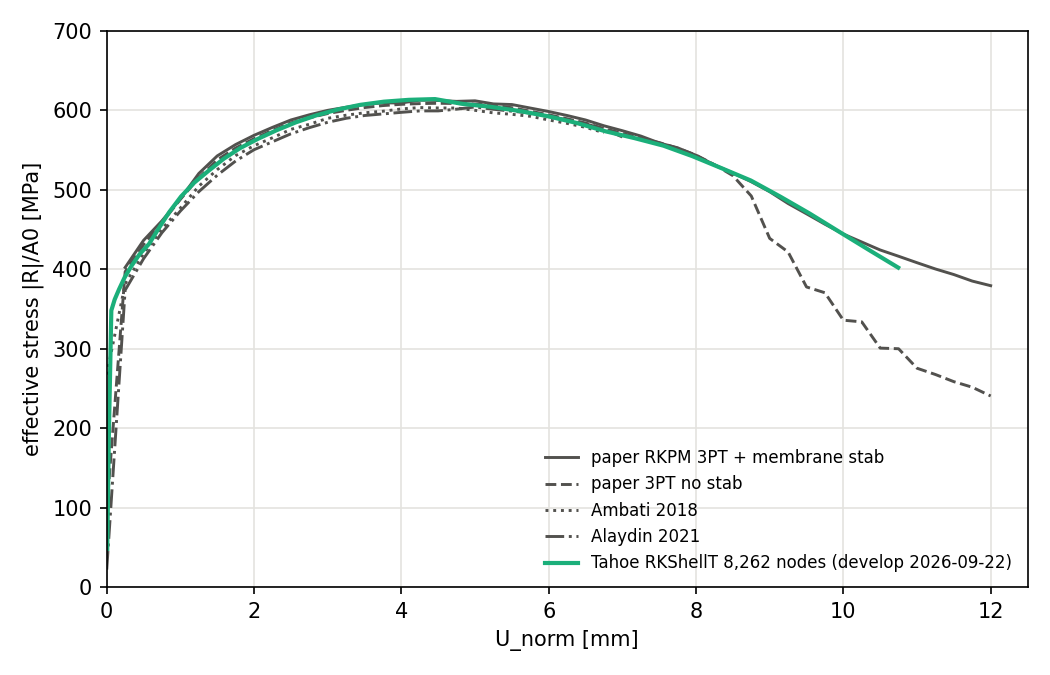
\includegraphics[width=0.82\textwidth]{necking_validation/fig15_compare.png}
\caption{Necking: Tahoe against the digitized paper Fig.~15.}\label{fig:necking}
\end{figure}

\begin{table}[h]
\centering\small
\begin{tabular}{@{}rrrr@{}}
\toprule
$U_{\mathrm{norm}}$ [mm] & Paper, 3 points + stabilization & Ambati et al.~\cite{Ambati2018} & Tahoe \\
\midrule
1 & 489 & 477 & 492 \\
2 & 569 & 555 & 564 \\
4 & 609 & 602 & 613 \\
6 & 598 & 588 & 593 \\
8 & 543 & -- & 542 \\
10 & 444 & -- & 447 \\
\bottomrule
\end{tabular}
\end{table}

The run follows the paper's stabilized curve from the elastic rise through the peak (614 against
609~MPa) and down the softening branch to $U_{\mathrm{norm}}=10.7$~mm, clearly separated from the
paper's unstabilized branch, which is near 300~MPa there. Beyond $U_{\mathrm{norm}}\approx10.9$~mm the
explicit run becomes unstable in the neck (Section~\ref{sec:limits}).

\subsection{Elasto-plastic pinched cylinder}\label{sec:pinch}
Cylinder $R=300$~mm, $L=600$~mm, $h=3$~mm, rigid diaphragms; $E=3000$~MPa, $\nu=0.3$,
$Y = 24.3 + 300\,\bar\varepsilon^p$~MPa; the two diametrically opposite mid-length points are driven
inward to 300~mm by the penalty controller, and the reported load is its multiplier $\lambda$.
Mass-scaled explicit dynamics, 50{,}000 steps, quasi-static past about 60~mm (kinetic energy below
5\% of the external work).

\paragraph{The load convention.} Every curve in the paper's Fig.~18 comes from, or matches, a
symmetry model: Ambati et al.~\cite{Ambati2018} model one quarter of the shell and Alaydin et
al.~\cite{Alaydin2021} one octant. In such a model the load point lies on two symmetry planes, so
the applied nodal force, which is what is plotted as the reaction, is one quarter of the physical
pinch load. For a long time this implementation appeared 4--9 times too stiff because its
physical load was compared with those curves directly.

\begin{figure}[h]
\centering
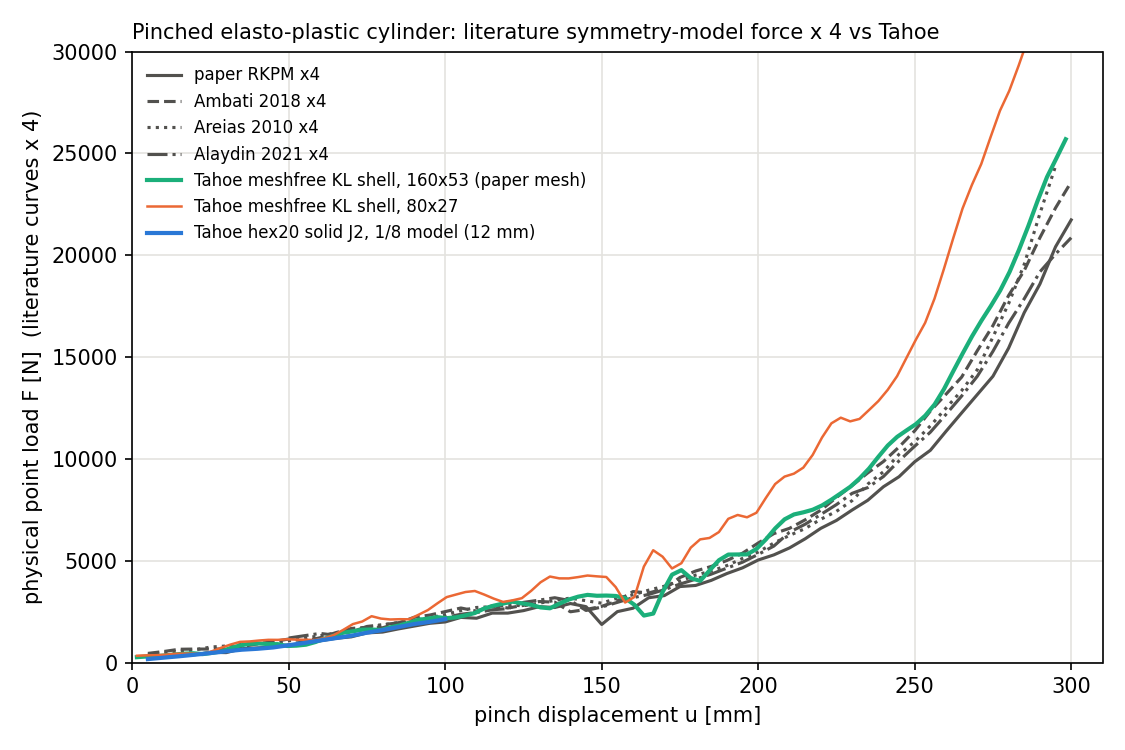
\includegraphics[width=0.85\textwidth]{fig18_validation/fig18_x4_overlay.png}
\caption{Elasto-plastic pinched cylinder: the published curves multiplied by 4 against the physical
point load from Tahoe's meshfree shell (two clouds) and an independent Tahoe hex20 solid model.}
\label{fig:pinch}
\end{figure}

\begin{table}[h]
\centering\small
\begin{tabular}{@{}rrrrrr@{}}
\toprule
$u$ [mm] & Paper $\times4$ & Ambati $\times4$ & Areias $\times4$ & Shell, 8{,}480 nodes & Solid, hex20 \\
\midrule
50 & 874 & 1156 & 1069 & 814 & 852 \\
100 & 1995 & 2502 & 2356 & 2182 & 2131 \\
200 & 5036 & 5870 & 5425 & 5580 & -- \\
300 & 21733 & 23595 & -- & 25692 & -- \\
\bottomrule
\end{tabular}
\end{table}

On the paper's resolution (160 by 53 nodes) the shell lies inside the band of the published results
over the whole crush and reproduces the load dip near 160~mm. An independent reference built from
Tahoe's finite-strain solid elements (one-eighth model, 20-node hexahedra, Simo $J_2$) agrees with the
shell to 100~mm and reproduces the linear obstacle-course deflection to 0.5\%. On the way to this
result the following were tested at the paper's resolution and excluded as causes of the apparent
mismatch: the boundary-condition treatment and the reported force, mesh resolution (a
33{,}600-node cloud agrees with 8{,}480 nodes within 5\%), the Taylor stabilization, and the end
conditions. Coarser clouds remain visibly too stiff (Fig.~\ref{fig:pinch}, 80 by 27 nodes).

% ===========================================================================
\section{Tests, benchmarks and continuous integration}\label{sec:tests}

\paragraph{Unit tests} (\code{tests/meshfree/}, Google Test, built with \code{TAHOE\_DEV=ON}):
shape functions on the chart (partition of unity, reproduction, derivative consistency), the
kinematic chain against finite differences, assembly (symmetry, rigid null space, patch tests),
stress update, plane-stress $J_2$ return, Scordelis--Lo through the in-memory element and through
the \code{tahoe} binary, the thickness update and co-rotation, and the collocation transform.

\paragraph{Regression benchmarks} (\code{benchmark\_XML}, compared with the \code{compare} tool):
\begin{itemize}[leftmargin=*]
  \item \code{level.0/meshfree\_kl\_shell}: Scordelis--Lo on the paper's 315-node cloud, the
  hemisphere and linear pinched cylinder, the collocation boundary condition, and the penalty
  displacement controller on the explicit and implicit paths.
  \item \code{level.2/meshfree\_kl\_shell}: shortened, mass-scaled versions of the necking
  cylinder and the elasto-plastic pinched cylinder (about 45~s each on one thread).
\end{itemize}
The validation decks and scripts behind Section~\ref{sec:vv} are in
\code{docs/meshfree\_kl\_shell/fig18\_validation} and \code{necking\_validation}.

\paragraph{Continuous integration and solver verification.}
Three GitHub Actions workflows build and test every push and pull request to \code{develop} and
\code{master}: a serial build (SPOOLES and SuperLU), a MUMPS build, and an MPI build. Each runs the
Google Test suite; the serial and MUMPS workflows then run benchmark levels 0--2 and the MPI
workflow level~3 on four ranks. A benchmark step fails only on a crash or timeout; comparison
failures are reported but tolerated, because level~0 carries a known set of legacy failures
(issue \#37).

From 21 to 25 September 2026 all three workflows failed on one unit test: the pipeline test ran a
Scordelis--Lo deck from the untracked personal \code{applications/} directory, which does not exist
on a CI runner. The test now runs the tracked level~0 deck. Before merging, the four configurations
below were built from scratch and tested locally; the first three reproduce the CI workflows.

\begin{table}[h]
\centering\small
\caption{Pre-merge verification, 25 September 2026.}\label{tab:ci}
\begin{tabular}{@{}lllll@{}}
\toprule
Configuration & Unit tests & Level 0 & Levels 1 / 2 & Level 3 (4 ranks) \\
\midrule
Serial (SPOOLES, SuperLU) & 95 / 95 & 173 pass, 0 crash & 103 / 103, 49 / 49 & -- \\
MUMPS & 95 / 95 & 173 pass, 0 crash & 103 / 103, 49 / 49 & -- \\
MPI & 95 / 95 & -- & -- & 22 / 22 \\
All solvers (MPI, MUMPS, METIS, SPOOLES-MT, SuperLU) & 95 / 95 & -- & -- & 22 / 22 \\
\bottomrule
\end{tabular}
\end{table}

The benchmark references cover the default solvers only, so the other solvers were
cross-validated: the same problem was solved with every solver and compared with SPOOLES. The
problems were an 18{,}000-degree-of-freedom nonlinear electro-mechanical liquid inclusion (27 Newton
iterations), a large-strain $J_2$ patch (6 iterations, 224 nodal values) and a linear diffusion bar.
SuperLU, serial MUMPS, SPOOLES-MT with 4 threads, and SPOOLES-MPI and MUMPS-MPI on 2 and 4 ranks,
each with METIS and with the built-in bisection partitioner, all reproduce the SPOOLES Newton
history (identical iteration counts, residuals within $2\times10^{-6}$ relative) and its nodal
output to machine precision ($<10^{-15}$ relative). Two exceptions were found. The profile (skyline)
solver is correct but too slow for the 18{,}000-degree-of-freedom problem. SPOOLES-MPI fails when the
10-node diffusion bar is split over four ranks, one of which owns a single equation; MUMPS-MPI solves
the same partition correctly.

One regression deck, \code{level.1/.../material.120/wlc\_superlu.xml}, aborts at step 11 of 290 with
every solver, identically before and after these merges, yet is counted as passing: it has no
stored reference and \code{tahoe} returns exit code 0 after a solver exception. Checking the run log
for exceptions in \code{run\_benchmarks.sh} would expose such cases.

% ===========================================================================
\section{Limitations and outlook}\label{sec:limits}

\begin{itemize}[leftmargin=*]
  \item \textbf{Deep necking.} The explicit necking run becomes unstable at
  $U_{\mathrm{norm}}\approx10.9$~mm, with a plastic strain of 1.28 and the thickness at 45\% of its
  initial value in a 3.75~mm band; the paper continues to 12.2~mm and strains near 2. Candidates are
  the stable time step at reduced thickness, the Pad\'e thickness update near its pole, and the
  scaling of the stabilization with the current thickness.
  \item \textbf{Membrane locking} (issue \#68). Coarse clouds are too stiff on inextensional bending
  (the 80 by 27 elasto-plastic pinched cylinder; the linear pinched cylinder at 0.71 of the
  reference on 1{,}260 nodes where the paper reaches 0.89). The
  paper's Section~5 sketches remedies; a patch-test-preserving stress projection in the spirit
  of~\cite{Belytschko1985} is the classical alternative. Two naive lower-order membrane projections
  were tried and did not soften the response.
  \item \textbf{Implicit plasticity.} Static elasto-plastic runs use the elastic stiffness and slow
  down once yielding spreads. A consistent or numerical tangent would make quasi-static shell
  plasticity cheap and remove the reliance on mass-scaled explicit runs.
  \item \textbf{Cubic completeness} reduces locking statically but is unstable with the lumped mass in
  explicit dynamics.
  \item \textbf{Quasi-uniform clouds.} One global spacing sizes all kernels; locally refined clouds
  need per-node support sizes.
  \item \textbf{Bending stabilization} is required for the thin hemisphere and is not part of the
  paper's formulation; self-contact and patch coupling are not yet validated on a full problem.
\end{itemize}

% ===========================================================================
\begin{thebibliography}{9}
\bibitem{WangBazilevs2025}
J.~Wang and Y.~Bazilevs.
\newblock A general-purpose meshfree Kirchhoff--Love shell formulation.
\newblock \emph{Engineering with Computers}, 41:1379--1410, 2025.

\bibitem{Ambati2018}
M.~Ambati, J.~Kiendl, and L.~De~Lorenzis.
\newblock Isogeometric Kirchhoff--Love shell formulation for elasto-plasticity.
\newblock \emph{Computer Methods in Applied Mechanics and Engineering}, 340:320--339, 2018.

\bibitem{Alaydin2021}
M.~D.~Alaydin, D.~J.~Benson, and Y.~Bazilevs.
\newblock An updated Lagrangian framework for isogeometric Kirchhoff--Love thin-shell analysis.
\newblock \emph{Computer Methods in Applied Mechanics and Engineering}, 384:113977, 2021.

\bibitem{Belytschko1985}
T.~Belytschko, H.~Stolarski, W.~K.~Liu, N.~Carpenter, and J.~S.-J.~Ong.
\newblock Stress projection for membrane and shear locking in shell finite elements.
\newblock \emph{Computer Methods in Applied Mechanics and Engineering}, 51:221--258, 1985.
\end{thebibliography}

\end{document}
